\documentclass{report}
\usepackage{graphicx}% Include figure files
\pagestyle{myheadings}
\markright{Lafe Spietz\hfill}
\begin{document}
\title{Practical Noise Measurement Near the Quantum Limit}
\author{Lafe Spietz}
\date{2017}
\maketitle

\section{Introduction}
	Noise temperature of microwave measurements near the quantum limit is becoming an increasingly critical issue in quantum information science.  Building and deploying ultra-low-noise amplfifiers is a key component to improving overall performance of this field, however simply building better amplifiers is not enough.  In order to realize the full potential of better amplifiers, as well as to continue to push the amplifier field ahead, quality measurements of noise are needed.   Many times multiple labs will buy the exact same amplifier only to find that one lab has twice the measured noise performance as another because of details of the measurement chain.  In this application note we discuss the physics and engineering needed to accurately measure the noise of a measurement chain.

\section{Noise Temperature}
	\subsection{Noise Temperature at High Temperatures}
		For the purpose of this application note, all components are assumed to be impedance matched to a 50 $\Omega$ transmission line.  We start by discussing very briefly how noise temperature is defined for amplifiers well above the quantum noise limit at temperatures well above the quantum temperature(both of these will be defined below). 

	In this high temperature regime it makes sense to define noise temperature the following way:  the noise temperature of an amplifier is the temperature of a matched load at the input the thermal noise of which exactly doubles the noise observed at the output.  For example, if an amplifier has 20 dB of gain and a 10 K noise temperature and a 10 K matched load were at the input one would measure a noise power at the output of 2000 K, or 10 K for the load plus 10 K for the amplifier times 100 for the power gain.  This definition is both aesthetically pleasing and simple to understand experimenatally.  As we shall see, however it is non-useful at very low noise levels and has led to decades of confusion.  

	One important point to note about this noise temperature is that it is a completely fictitious temperature.  There is no implied object in the amplifier which is actually physically at the noise temperature.  A room temperature amplifier can, for instance, have a noise temperature of just a few 10's of kelvin.  Temperature units are used because they are convenient way to describe white noise and because they are easy to think about in the context of both low temperature physics and radio astronomy, but they should not be taken too seriously as a physical property(although, confusingly, noise temperatures often scale linearly with temperature).  

	\subsection{Noise Temperature Through a Measurement Chain}

	One subject that is constantly confusing for people who are new to amplfiier noise measurements is how to deal with system noise in a multi-section measurement chain.  Whether one is dealing with communications, radio astronomy or low temperature physics, the amplifier in question is never alone in the measurement chain.  There are generally cables, directional couplers, circulators, multiple stages of amplifier, attenuators, as well as various impedance mismatches.  

	The most important of these cases is that of multiple stages of amplifier.  When analyzing a chain of amplifiers, the key fact is that one must multiply by linear power gain going forward in the chain and divide by linear power gain going backward through the chain.  In quantitative terms, if a pair of amplifiers have gains $G_1$ and $G_2$ and noise temperature $T_{n1}$ and $T_{n2}$, the total gain is $G_1G_2$ and the total noise temperature is $T_{n1} + T_{n2}/G_1$.  Note that if the gain of the first stage amplifier is high, the noise of the second stage has very little affect on the overall noise of the combined amplifier chain.  For instance if a cryogenic amplifier has 40 dB of gain, if the following amplifier at room temperature has 10,000 K noise temperature it only adds 1 K of noise to the total measurement chain!  This shows why the first stage is so much more critical than any other part of the measurement chain.  If the first stage has high enough gain and low enough noise, the demands for noise on the rest of the chain can be relatively low.  

	Most other impedance-matched elements which add loss can be modelled as attenuators, so we consider those next.  An attenuator with linear attenuation factor A may be considered to be an amplifier with power gain less than one (G = 1/A), with a noise temperature equal to the physical temperature times A - 1.  The noise temperature of a amplfiier with an attenuator at its input is then $T^{attenuator}_n + AT^{amplifier}_{n} = T^{attenuator}_{physical}(A-1) + AT_n^{amp}$, where A is the linear power attenuation, $T^{attenuator}_{physical}$ is the physical temperature of the attenuator, and $T_n^{amplifier}$ is the amplifier noise temperature.  This is why minimizing loss at the input of an amplifier chain is so critical.  For example, a 3 dB loss at the input of an amplifier, even if it is at a negligible temperature, adds a factor of at least 2 if not more(depending on the attenuator temperature, which could add another factor of 2 or more) to the overall system noise temperature!  It is quite common for low temperature physicists using exactly the same cryogenic low noise amplifier to see as much as a factor of four difference in observed system noise temperature due to small differences in how microwave loss is handled for this reason.  

	\subsection{Quantum Noise of a Resistor}

	Althought it is described at length in the literature it is worth describing here the nature of noise from a impedance-matched resistor including quantum mechanical effects, because we will rely on that extensively in this dicsussion.  The noise power $S_I50 \Omega$ (in Watts per Hz, which has units of energy) from a matched load at temperature T and angular frequency $\omega$ is
\begin{equation}
P(\omega,T)=\frac{\hbar\omega}{2}\coth{\left(\frac{\hbar\omega}{2kT}\right)}.
\end{equation}

Note that in the limit of high temperature and low frequency is kT.  In the limit of low temperature and high frequency $\frac{\hbar\omega}{2}$.  For the purpose of this discussion we prefer to use units of photons per mode rather than power.  To convert to photons per mode we divide energy by $\hbar\omega$, to get the ``noise number'', 
\begin{equation}
n(\omega,T)=\frac{1}{2}coth{\left(\frac{\hbar\omega}{2kT}\right)}.
\end{equation}


	\subsection{Historical Background and Erroneous Definitions}

	Before defining the noise units we will use we must discuss some of the erroneous definitions of noise temperature which exist in the literature and cause extensive confusion.  One of the major sources of confusion is the high temperature definition used above in this note.  Defining the noise temperature in terms of the \textit{temperature} of a load at the input of the amplifier becomes highly problematic in the case where kT is near $\hbar\omega$.  Naive application of this exact definition has led to several non-useful definitions for the quantum limit and for noise temperature.  By solving for the temperature of a quantum resistor in the above expression, some authors have used definitions of noise temperature which are not linear in the amplifier noise power, and which add factors of either $\ln{2}$ or $\ln{3}$ depending on whether the vacuum noise is ignored or not.  Furthermore, there are authors who rather than ignore the vacuum noise, count it twice, including both the added noise of the amplifier and the quantum noise of the matched load in the total stated noise, adding a factor of 2 to the classical definition above.  It is not our purpose to delve deeply into the literature here to account for all the published errors.   However, we wish to warn the reader that grievous errors and inconsistencies exist in parts of the amplifier literature both from physics and from engineering journals, and that great care must be taken when attempting to interpret the results of some papers.  

	\subsection{Proper Units for Quantum Amplfiier Metrology}

	Due to the level of confusion in the literature, great care must be taken in defining the units for measuring amplifier noise.  The unit we describe here is one which we claim is used colloquially by almost the entire amplifier community but which is almost never stated explicitly.  Often the incorrect definition used above is stated in the same paper where in the body of the paper a more consistent definition is used in practice.  

	We define the noise temperature of an amplifier by considering a amplifier with a matched load at the input such that the noise at the output is half from the load and half from added amplifier noise.  In this situation, 
\begin{equation}
T_N = \frac{P}{2kG},
\end{equation}
	where P is the noise power per unit of bandwidth measured at the output of the amplifier, G is the linear power gain of the amplifier and k is the Boltzmann constant.   In the situations where the noise from the resistor is completely thermal, this definition is identical to the classical definition.  But it has the important difference that as we get into the quantum regime the noise temperature in kelvin units continues to be linear in added noise power.  

	In addition to noise temperature and noise number we now mention a third unit which is used in the amplifier industry, the noise figure.  The noise figure is a way of comparing noise temperature to 290 K, expressed in dB.  Thus the noise figure NF is 
\begin{equation}
NF = 10 \log{\left(1 + \frac{T_N}{290}\right)}.
\end{equation}

While this figure of merit is not very useful at low temperatures and is less favored by phycisists than engineers, it is important to include it here for completeness.  Many amlifier companies specify their amplifiers in noise figure and being able to quickly compare this to noise temperature is useful.  To that end, we include here a short table comparing noise figure, noise temperature, and noise number at 5 and 10 GHz.  

\begin{center}
    \begin{tabular}{ | l | l | l | l |}
    \hline
    Noise Temperature [K] & Noise Figure [dB] & n(5 GHz) & n(10 GHz) \\ \hline
    0.05 & 0.00075 & 0.21 & .10 \\ \hline
    0.1 & 0.0015 & 0.42 & 0.21 \\ \hline
    0.5 & 0.0075 & 2.1 & 1.0\\ \hline
    1 & 0.015 & 4.2 & 2.1\\ \hline
    4 & 0.059 & 17 & 8.3\\ \hline
    10 & 0.15 & 42 & 21\\ \hline
    40 & 0.56 & 170 & 83\\ \hline
    80 & 1.1 & 330 & 170\\ \hline    
    100 & 1.3 & 420 & 210\\ \hline
    290 & 3.0 & 1200 & 600\\ \hline
    1000 & 6.5 & 4200 & 2100\\ \hline

    \end{tabular}
\end{center}
	
There are a couple of things worth noting about these numbers.  First of all note that this noise number is, as we will see below, not the factor by which the amplifier's noise is above the quantum limit.  An amplifier with a noise number of 1 is twice the quantum limit rather than exactly at the quantum limit.  Second of all, the noise number is, as with noise temperature, \textit{added} noise from the amplifier, not the total noise referenced to the input.  If the input is a matched load in equilibrium at zero temperature, it will add at least 1/2 to the observed noise referenced to the input.  One of the errors in some papers in the literature is including this 1/2 in the quantum limit, while still mixing units with temperature units.  Again, always be careful to determine which of the various definitions the author of any given paper is using.

\subsection{Quantum Limits of Amplifiers}

	There is a Heisenberg uncertainty relation between the two phase quadratures of a measurement of a quantum signal. We will not delve into the physical details of this here, and they are very thoroughly covered in the references(ref).  We will only state the relevant limits on amplifiers from an engineering perspective.  

	We first define the somewhat confusing standard nomenclature used in the literature.  ``Phase insensitive'' refers to amplifiers that amplify a signal without regard to the phase of the signal.  This describes almost all commercially available and high temperature amplifiers, as well as amplifiers based on the DC-SQUID and the non-degenerate parametric amplifier.  ``Phase sensitive'' amplifiers have gain which is different for the different phase quadratures.  This applies to degenerate parametric amplifiers.  This distinction is critical from an engineering perspective, because when gain depends on phase it is possible to measure one of the quadratures with arbitrary precision by throwing away precision in the other quadrature.  

	For phase insensitive amplifiers, the uncertainty relation implies the following limit on the noise number n:
\begin{equation}
n\geq \frac{1}{2}\left|1 - \frac{1}{G}\right|, 
\end{equation}
where G is the power gain of the amplifier.  Note that if the gain is 1, as for a lossless transmission line, no noise must be added.  For large gains, this relation means that all phase insensitive amplifiers must add at least half a photon of noise per mode.  Translating this into a minimum possible noise temperature in kelvin at different frequencies is useful, and we do that in the follwing table.  
\begin{center}
    \begin{tabular}{ | l | l  |}
    \hline
    Frequency [GHz] & Quantum Limit [mK] \\ \hline
    0.25 & 6  \\ \hline
    0.5 & 12  \\ \hline
    1 & 24 \\ \hline
    2 & 48 \\ \hline
    4 & 96\\ \hline
    8 & 192 \\ \hline
    16 & 384\\ \hline
    \end{tabular}
\end{center}

It is worth noting that as with measuring position without momentup or energy without phase, if we only measure one phase quadrature there is no quantum limit on the precision.  This allows us to use the troubling phrase ``below the standard quantum limit'' to describe the performance of amplifiers which have a noise in one quadrature below half a photon per mode.  This can be very useful for measurement of harmonic signals where the phase of the signal is known and one does not need any information from the other quadrature.  Note that if the harmonic signal is not squeezed, that there is still always a half photon added from the quantum noise from the signal, so squeezing of this signal would be useful to get the ultimate maximum possible precision in measurement.  

\section{Microwave Measurement and Amplifier Noise}
	\subsection{White Noise and Measurement}
		
	Here we discuss the effect of amplifier noise on practical measurement time.  When measuring an effective temperature T with added noise $T_n$, the imprecision in the measurement in temperature units is given by the Dicke radiometer formula
\begin{equation}
\delta T = \frac{T + T_n}{\sqrt{B\tau}},
\end{equation}
where B is the bandwidth of the measurement and $\tau$ is the integration time.  This formula is important since it shows the power of noise temperature in determining integration time.  If we assume that we want a fixed signal to noise ratio, and that amplifier noise dominates the overall noise, the time required to achieve that signal to noise ratio scales with the \textit{square} of the noise temperature.  Thus even a factor of order 3 improvement in noise temperature can shorten integration times by a factor of 10 to get the same performance.  Note that this consideration also applies to measurement of harmonic signals with no added noise, since the white noise background from the amplifier still integrates down according to this formula.  

We briefly digress to discuss how to estimate noise thermometer performance.  By simply substituting the estimated temperature and noise temperature and bandwidth into the above formula, we can get a total number for temperature uncertainty in K/$\sqrt{Hz}$, which makes estimation of measurement times and errors simple.  For instance in a typical microwave noise thermometry measurement with 10 K of added noise and 100 MHz bandwidth, the uncertainty is about 30 mK/$\sqrt{Hz}$

	\subsection{Amplifier Noise and Qubit Fidelity}

\section{Measurement System Noise}
	\subsection{Concatenation of Elements of a Measurement Chain Near the Quantum Limit}
		
	The discusssion above of dealing with chains of components in series needs modification when dealing with quantum effects.  Dealing with amplifiers is the same, as long as we are careful to use the appropriate noise units.  Attenuators are a special case, however, since the added noise from the loss must be treated with the full quantum expression.  The noise number of a attenuator is
\begin{equation}
n_{att} = \left(\frac{1}{G} - 1\right)\frac{1}{2}\coth{\frac{\hbar\omega}{2kT}}, 
\end{equation}
in direct extension to the classical case above.  Note that this means that in a dilution refrigerator at microwave frequencies, the dominant added noise source from any lossy element is the quantum noise.  



%	\subsection{Reflections}


\section{Practical Noise Determination}
	\subsection{Y-Factor Measurement}

	The Y-factor method invovles measuring the output noise of a measurement system at two known temperatures and calculating the noise and gain from those noise values.  This is generally used in the classical regime where noise depends linearly on temperature.  In the classical regime, we consider the output noise to be $P_{1,2} = G(T_n + T_{1,2})$, where G is gain in units of output power per kelvin of noise, $T_n$ is amplifier noise temperature, and $T_{1,2}$ are the two physical temperatures.  It is then straight foward to compute the noise temperature from two noise power measurements.  
\begin{equation}
T_n = \left(\frac{T_2 - T_1}{P_2 - P_1}\right)P_1 - T_1.
\end{equation}

	This method has several problems for people doing measurements near the quantum limit.  First of all, if both temperatures are in the quantum regime there is very little difference in noise power.  At 10 GHz, a 10 mK load and a 20 mK load are almost identical in noise power, for instance, and much higher temperatures are needed to get any useful data.  In the quantum case, we can write the photon number noise at the output as $P_{1,2} = G(n + \frac{1}{2}\coth{\frac{\hbar\omega}{2kT}})$.  This yields the following awkward formula for noise number
\begin{equation}
n = \left(\frac{\frac{1}{2}\coth{\left(\frac{\hbar\omega}{2kT_2}\right)} - \frac{1}{2}\coth{\left(\frac{\hbar\omega}{2kT_1}\right)}}{2(P_2 - P_1)}\right)P_1 - \frac{1}{2}\coth{\left(\frac{\hbar\omega}{2kT_1}\right)}.
\end{equation}

	Given that at very low temperatures the noise levels of different temperatures are almost identical, one needs to have one temperature be much higher than the other to get over the quantum temperature.  Heating to significant fractions of a kelvin or over a kelvin in a dilution refrigerator can be very disruptive and can lead to errors due to excessive heating.  Also, going from one stable temperature to another in a low temperature apparatus can be very time consuming, and when large numbers of data points are needed to characterize the noise of an amplifier, this can lead to huge time investments.  

	\subsection{Room Temperature Noise Measurements}
	
	Another very common method of measuring noise is to use a calibrated active noise source.  There are a variety of commercially avialable sources used for this purpose.  The commercial sources which are widely available are at room temperature.  This neccesitates using both extensive attenuators and cables to get from the source to the input of the cryogenic amplifier, with the number of components increasing as the amplifier gets closer and closer to the quantum limit.  The final accuracy of the noise at the input of the amplifier is then dependent on knowing the exact attenuation and temperature of every stage of the measurement chain from the source to the amplifier.  While these kinds of systems can be very efficient for noise calibration at room temperature and at moderate cryogenic temperatures they are extremely impractical for ultra-low-noise cryogenic amplifiers near the quantum limit.  

	\subsection{Shot Noise Sources}
	

	The problems listed above with standard noise calibration techniques are solved by using the various shot noise sources which are available.  Shot noise sources can be very close to the input of the amplifier, can by compact and can work at any temperature.  They can allow for very rapid and accurate measurement of noise.  Some subtleties must be understood, however, if the accuracy is to be realized.  

	The primary device we will discuss here is the Shot Noise Tunnel Juntion(SNTJ).  This device is a matched 50 $\Omega$ load where the origin of the resistance is a tunnel junction.  By applying a DC bias current to the junciton and measuring the voltage, it is possible to have a very accurate knowledge of the noise based on well-understood physics.  

\begin{figure}
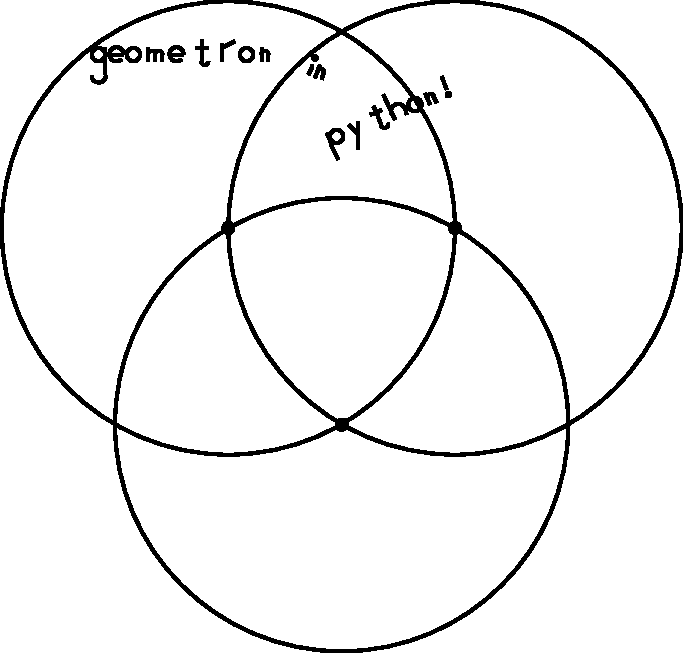
\includegraphics{foo2.pdf}
\caption{Quantum noise.  Green dotted lines show asymptotes of linear shot noise and blue lines indicate bottom of noise curve and the top of the amplifier noise level.  As an example, the following is a plot of normalized noise with an amplifier at three times the quantum limit, or n = 1.5, and for t = 0.09, which would be for a 30 mK fridge and a 7 GHz signal.}
\end{figure}

 	For a tunnel junction at finite frequency, the output noise number is 
\begin{equation}
n_{SNTJ} = \frac{1}{4}\left( u + 1\right)\coth{\left(\frac{u+1}{2t}\right)} + \frac{1}{4}\left( u - 1 \right)\coth{\left(\frac{u-1}{2t}\right)} ,
\end{equation}
where u is the normalized voltage $\frac{eV}{\hbar\omega}$ and t is the normalized temperature $\frac{kT}{\hbar\omega}$. In the limit of low frequency and high temperature, this expression reduces to 
\begin{equation}
n_{SNTJ} = \frac{1}{2}u\coth{\left(\frac{u}{2t}\right)} = \frac{eV}{2\hbar\omega}\coth{\left(\frac{eV}{2kT}\right)}, 
\end{equation}
or
\begin{equation}
T_{SNTJ} = \frac{eV}{2k}\coth{\left(\frac{eV}{2kT}\right)}
\end{equation}

By measuring the noise at the output of the measurement chain at several voltages, one may readily determine the full system noise temperature or noise number.  This can be done by either measuring two points in the fully linear range of the curve or by measuring a larger number of points and fitting them to the functional form above.  The plot of normalized noise number at the output of the amplifier shows conceptually how the added noise from the measurement manifests itself as an offset in the curve.  Since the bias point can be changed in a very small fraction of a second, it is possible for low noise amplfiers to acquire noise data as a function of various parameters very quickly.  

The equation for the noise number at the output of the whole measurement chain is
\begin{equation}
n = G(n_{amp} + n_{SNTJ}),
\end{equation}
where $n_{amp}$ is the added noise number from the amplifier and $n_{SNTJ}$ is as defined above.  Looking at typical theoretical noise curve plotted here we see that all of the information about temperature is in the voltage range where $eV\approx\hbar\omega$.  Below that voltage, there is very little information about either amplifier noise or temperature.  A straightforward way to measure noise temperature or noise number is to measure the noise at two voltages, both on the linear range of the curve.  Good choices for an accurate linear measurement are(cite thesis) $(\hbar\omega + 5 kT)/e$ and $(\hbar\omega + 10 kT)/e$.  This is very much like a y-factor measurement.  

	In this regime, the noise number from the junction is 
\begin{equation}
n_{SNTJ} =  \frac{1}{2}u,
\end{equation}
and the noise temperature is 
\begin{equation}
T_{SNTJ} = \frac{eV}{2k},
\end{equation}
so from two points both on the linear regime, if we measure output noises $n_1$ and$n_2$, the added system noise number is 
\begin{equation}
n_{system} = \frac{u_2 -  u_1}{n_2 - n_1}n_2 - \frac{1}{2},
\end{equation}
and the added system noise temperature is 
\begin{equation}
T_{system} = \frac{eV_2 - eV_1}{2kT_2 - 2kT_1}T_2 - \frac{\hbar\omega}{2k}.
\end{equation}

	With a shot noise source in hand, writing data acquisition code to get these numbers quickly is relatively straigthforward.  Note that in the quantum regime it is important to use the frequency-appropriate formula for each frequency.  
	
	Detailed instructions for constructing junctions of this kind are published elsewhere, but for the purpose of this application note the reader may assume that the devices are provided fully functional over the desired range of measurement.  The shot noise junctions and capsules designed and fabricated by the author have minimal loss and excellent coupling to over 12 GHz and are easy to heat sink to cold plates with arbitrary hole patterns.

\end{document}
